\documentclass[12pt,a4paper]{article}
\usepackage[utf8]{inputenc}
\usepackage[english]{babel}
\usepackage[T1]{fontenc}
\usepackage{amsmath}
\usepackage{amsfonts}
\usepackage{amssymb}
\usepackage{graphicx}
\usepackage{siunitx}
\usepackage{float}
\usepackage[left=2cm,right=2cm,top=2cm,bottom=2cm]{geometry}
\author{Gerald}

\begin{document}
\sisetup{separate-uncertainty = true}
	\setlength{\parindent}{0pt} 
	\begin{center}
		{\LARGE Experiment protocol}\\
		\begin{large}
			for the solid state lab course\\[0.4cm]
			at RWTH Aachen\\
			II. Physikalisches Institut A\\[5.5cm]
			\Large\textbf{\textsl{Superconductivity and SQUID}}\\[5.5cm]
			\normalsize\textit{authored\\by}\\[0.4cm]
			\large{Moritz Berger (355244)\\Gerald Kolter (355005)}\\[2cm]
			\large \textbf{Summer term 2019}
		\end{large}
	\end{center}
	\newpage
	
	\tableofcontents
	\newpage

\section{Introduction}
Superconducting Quantum Information Devices ("SQUIDS") are very sensitive sensors for magnetic flux. A SQUID consists of a ring shaped superconductor with two contacts and each one Josephson junction on each path between the contacts. A Josephson junction is a small insulator between two superconductors. Electrons can tunnel through the insulator as Cooper pairs. \\
The resolution of the measured magnetic flux is in the order of the so called fluxonium or flux quantum:
\begin{equation*}
\Phi _0 = \dfrac{h}{2e} = 2 \times 10^{-15}\si{Wb}
\end{equation*}


\section{Goal of the Experiment}
The goal of the experiment is to first determine the critical temperature of the superconducting material $T_C$. \\
With the SQUID cooled down to the superconducting regime one measures the voltage-current characteristic. From this one can determine the critical current $I_C$, the resistance in the normal conducting state $R_N$ and the characteristic voltage $V_C$. \\
Next one measures the voltage-magnetic flux characteristic. From this one determines the SQUID parameter $b_L$ given by:
\begin{equation}
b_L = 2 \cdot I_C \cdot \dfrac{L}{\Phi _0}
\end{equation}
And with that the magnetic flux quantum $\Phi _0$. \\
With bringing different metallic objects in the vicinity of the SQUID one can demonstrate the sensitivity of the SQUID to external magnetic fields. This is done with and without the metallic shielding of the SQUID.


\section{Setup}
The setup consits of a SQUID in a metallic tube, which shields external magnetic fields. This setup is called "Mr. SQUID" and selled by the company "Conductus". The SQUID is sinked in a dewar filled with liquid nitrogen to cool it down to the necessary temperatures. \\
The SQUID itself is build out of Yba$_2$Cu$_3$O$_{7-x}$ with $x \approx 0-0.2$. The temperature is measured with a Pt-100 resistor.


\section{Measurement}
\section{Data}
\section{Results and Discussion}
\section{Conclusion}


%\begin{figure}
%\centering
%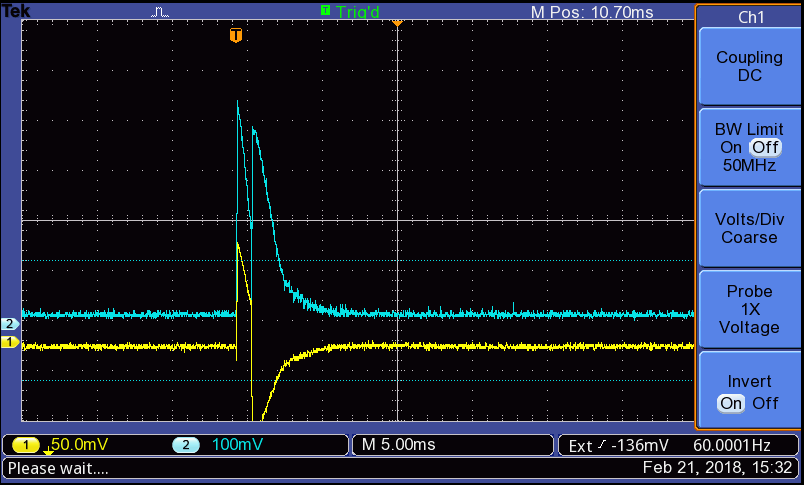
\includegraphics[scale=0.8]{Bilder/F0003TEK.PNG}
%\caption{Ergebnis einer einzelnen Messung zur Bestimmung von T1. Die blaue Kurve zeigt das zu untersuchende Signal.}
%\label{fig:MessungT1_Beispiel}
%\end{figure}



%\begin{table}
%\centering
%\begin{tabular}{|c|c|c|}
%\hline 
%Pulshöhe [mV] & FID-Höhe [mV] & $\tau$ [ms] \\ 
%\hline 
%428 $\pm$ 4 & -376 $\pm$ 4 & 0.918 $\pm$ 0.042 \\ 
%\hline 
%432 $\pm$ 4 & -360 $\pm$ 4 & 1.800 $\pm$ 0.042 \\ 
%\hline 
%432 $\pm$ 4 & -336 $\pm$ 4 & 2.700 $\pm$ 0.042 \\ 
%\hline 
%452 $\pm$ 4 & -308 $\pm$ 4 & 3.618 $\pm$ 0.042 \\ 
%\hline 
%452 $\pm$ 4 & -276 $\pm$ 4 & 4.554 $\pm$ 0.042 \\ 
%\hline 
%432 $\pm$ 4 & -248 $\pm$ 4 & 5.436 $\pm$ 0.042 \\ 
%\hline 
%440 $\pm$ 4 & -216 $\pm$ 4 & 6.300 $\pm$ 0.042 \\ 
%\hline 
%428 $\pm$ 4 & -184 $\pm$ 4 & 7.290 $\pm$ 0.042 \\ 
%\hline 
%440 $\pm$ 4 & -156 $\pm$ 4 & 8.154 $\pm$ 0.042 \\ 
%\hline 
%436 $\pm$ 4 & -116 $\pm$ 4 & 9.036 $\pm$ 0.042 \\ 
%\hline 
%436 $\pm$ 4 & -104 $\pm$ 4 & 9.954 $\pm$ 0.042 \\ 
%\hline 
%432 $\pm$ 4 & -72 $\pm$ 4 & 10.854 $\pm$ 0.042 \\ 
%\hline 
%424 $\pm$ 4 & -52 $\pm$ 4 & 11.862 $\pm$ 0.042 \\ 
%\end{tabular} 
%\caption{Messwerte der Höhen des $\pi /2$-Pulses und des FID s beim Durchfahren von $\tau$ zur Bestimmung von T1.}
%\label{tab:T1_Daten}
%\end{table}



\end{document}